% !TEX spellcheck = en_US

\documentclass[conference]{IEEEtran}
\usepackage{cite}
\usepackage{amsmath,amssymb,amsfonts}
\usepackage{algorithmic}
\usepackage{graphicx}
\usepackage{textcomp}
\usepackage{xcolor}
% add hyperlinks, delete all .aux files if adding hyperref after previous build
\usepackage{hyperref}
% support for unicode charcters like "é" and "ñ"
\usepackage[T1]{fontenc}
% Provides generic commands \degree, \celsius, \perthousand, \micro and \ohm
\usepackage{gensymb}
% splits a section into multiple columns
\usepackage{multicol}
\def\BibTeX{{\rm B\kern-.05em{\sc i\kern-.025em b}\kern-.08em
    T\kern-.1667em\lower.7ex\hbox{E}\kern-.125emX}}
\begin{document}

\title{Tracker Terrain Loss Part Two}

\author{\IEEEauthorblockN{Mark A. Mikofski, Mike Hamer, Anja Neubert, MinWah, Leung, Abhishek Parikh, and Rounak Kharait}
	\IEEEauthorblockA{DNV, Oakland, CA, 9612, USA }}

\maketitle

\begin{abstract}
Trackers on variable terrain can incur electric mismatch losses from row-to-row shading, even with backtracking. Standard and slope-aware backtracking algorithms only eliminate row-to-row shade for trackers on flat ground. Tracker terrain loss is the difference between the theoretically best performance of trackers on flat ground and the performance of trackers using standard backtracking algorithms but on variable terrain. We used SolarFarmer to study tracker terrain loss by simulating the Hopewell Friends Solar power plant, which has an average 4\% southwest slope. We calculated a tracker terrain loss of 2.4\% when the entire site was modeled as one layout for both 5-minute and 1-hour input data. By subdividing the site into two and three layouts, the tracker terrain loss decreased to 1.8\% and 1.6\% respectively. For this particular site, neither higher frequency input data nor slope-aware backtracking significantly affected the tracker terrain loss. This study is a continuation of a previous study that prompted improvements in SolarFarmer's 3-dimensional tracker shading algorithm. The results of this study demonstrate that SolarFarmer can now be used to calculate tracker terrain loss. In the final report we'll also compare SolarFarmer with another model developed at DNV.
\end{abstract}

\begin{IEEEkeywords}
trackers, terrain, losses, backtracking
\end{IEEEkeywords}

\section{Introduction}
Trackers increase energy output of PV systems by following the sun, maximizing the area of sunlight incident on the panels. However, most silicon modules are susceptible to electrical mismatch caused by uneven shade, therefore, trackers typically "backtrack" to avoid  row-to-row shade occurring after sunrise and before sunset. The tracking and backtracking algorithms for flat horizontal and sloped ground are described by closed-form expressions \cite{Marion2013,Anderson2020}, but there is no general solution for terrain with variable slopes. If the standard backtracking algorithms for flat ground are used for trackers on variable terrain, then row-to-row shading will occur, and therefore common silicon panels will incur electrical mismatch losses. The loss has been called the "tracker terrain loss" and can be expressed as the difference between the performance of trackers on flat versus variable terrain. Evaluating the tracker terrain loss is important because it can help determine if advanced tracker algorithms are necessary to reduce the risk of plant underproduction.

To study tracker terrain loss in detail, we used SolarFarmer \cite{Mikofski_8547323} because it can perform full 3-dimensional modeling of the shade and irradiance on the trackers in any position on any terrain and calculate full sub-module electrical mismatch to determine the performance of the PV system at each time step. This study is a continuation from last year \cite{Mikofski_9300381} in which we determined that the prior methods used in SolarFarmer were too coarse to resolve row-to-row shade for trackers during backtracking. Therefore, over the past year, a new hybrid 3-dimensional geometric shade algorithm was implemented in SolarFarmer to calculate the row-to-row shade on trackers at each time step exactly without any approximations. This paper presents the results of the new SolarFarmer methods applied to the same tracker simulations from last year, and expands on them slightly by testing both standard horizontal and slope-aware backtracking algorithms and running the simulations with both 5-minute and 1-hour input data resolution to determine if the tracker terrain losses are affected by either.

\section{Methods}

\subsection{Site Characteristics}

The Hopewell Friends Solar power plant is a single-axis array funded by the Department of Energy and built by Cypress Creek Renewables \cite{CypressCreekRenewables2019} near Asheboro, NC at a latitude and longitude of 35.627994$^\circ$ and -79.872853$^\circ$ respectively. The site is asymmetric, with 25-qty variable length rows of 2-in-portrait and 18-modules wide single-axis trackers. The modules are 1.978-meters long, and the rows are spaced about 7.8-meters apart, so the GCR is about 51\%. There are 18-qty Longi LR6-72BP-360 360-watt bifacial modules per string, and three strings per each Huawei SUN2000-25KTL-US 25-kW inverter. The inverters each have three inputs, so that's one string per input.

The terrain has a generally southwestern slope as shown in the contour map in Fig.~\ref{fig:hopewell_contour_map} with slightly steeper southern slopes on the east side of the array and milder western slopes on the north side of the array. The maximum and average slopes for each aisle from west to east in the array are summarized in Table~\ref{table:ew-slope-summary} starting with aisle 1 at the top northern tip of the array. The maximum and average north-south slopes for every 5 rows are shown in Table~\ref{table:row-slope-summary} starting with the 1st row on the western side of the array.

\begin{figure}[htbp]
\centerline{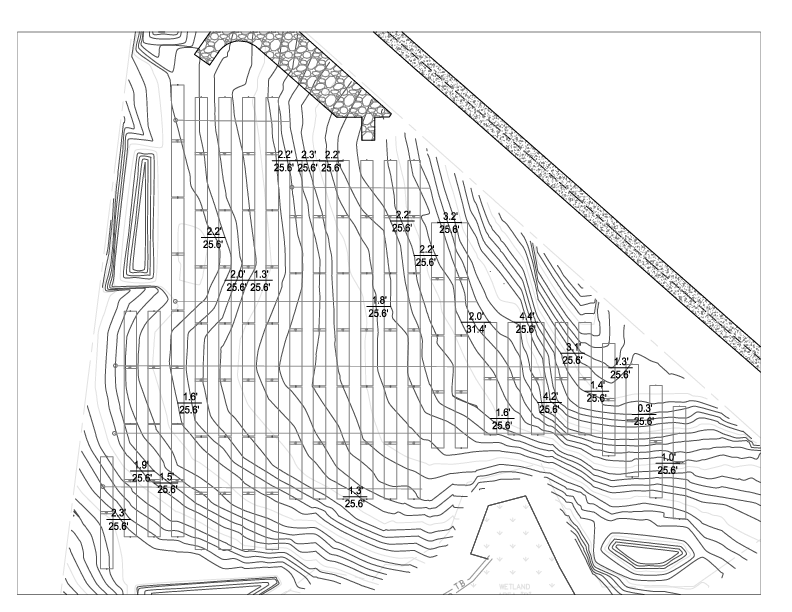
\includegraphics[width=9cm]{Hopewell_Civil_Base.png}}
\caption{Contour map of terrain at Hopewell, NC, single-axis array.}
\label{fig:hopewell_contour_map}
\end{figure}

\begin{table}[htbp]
\caption{Summary of East-West Slopes}
\begin{center}
\begin{tabular}{|c|c|c|c|}
\hline
\textbf{Aisle} & \textbf{\textit{Maximum}}& \textbf{\textit{Average}}& \textbf{\textit{Direction}} \\
\hline
1& 7.81& 6.22& west \\
\hline
2& 7.58& 6.59& west \\
\hline
3& 6.7& 5.77& west \\
\hline
4&5.99& 5.26& west \\
\hline
5& 5.08& 4.28& west \\
\hline
6& 4.69& 3.54& west \\
\hline
7& 4.42& 3.28& west \\
\hline
8& 4.06& 3.99& west \\
\hline
\end{tabular}
\label{table:ew-slope-summary}
\end{center}
\end{table}

\begin{table}[htbp]
\caption{Summary of North-South Slopes}
\begin{center}
\begin{tabular}{|c|c|c|c|}
\hline
\textbf{Row} & \textbf{\textit{Maximum}}& \textbf{\textit{Average}}& \textbf{\textit{Direction}} \\
\hline
1&  1.76&  1.11& south \\
\hline
5&  2.04&  1.77& south \\
\hline
10& 2.95&  2.54& south \\
\hline
15& 4.81&  4.35& south \\
\hline
20& 6.66&  5.84& south \\
\hline
25& 8.35&  4.96& south \\
\hline
\end{tabular}
\label{table:row-slope-summary}
\end{center}
\end{table}

\subsection{Model Simulation}

The system was modeled using SolarFarmer \cite{Mikofski_8547323} which allows parallel trackers to be oriented in any direction on any slope either in a plane or following the terrain. The Hopewell Friends Solar array was modeled with 111-qty trackers with a total of 222 strings for a total DC size of 1.44-MW, which is slightly smaller than the specified size of 1.45-MW. Also the modeled site has 74 inverters with a DC/AC ratio less than one to remove the effects of clipping, versus the actual site which has only 45 inverters and a DC/AC ratio of 1.3. Also the simulated tracker spacing is uniform throughout the array and the tracker aisles are aligned, which also differs from the site specifications. Finally the panels were treated as monofacial, because bifacial is currently only possible for 2-dimensional simulations, and for this study we needed to take advantage of 3-dimensional modeling to capture the terrain. These changes were made for ease of modeling and to make sure that variable row spacing and other artifacts did not affect the results, since we only want to observe the effect of slope.

Fig.~\ref{fig:layouts} shows how the site was modeled three times using a single layout, 2 layouts, and 3 layouts. As shown in Table~\ref{table:system-summary}, this results in layouts with different orientations, so they will track slightly differently. Each model was then simulated in both tracker placement modes to determine the tracker terrain loss. The "in-plane" mode positions all trackers in the same plane so there is zero row-to-row shading, but may result in some trackers exceeding the maximum specified height above the ground. The "follow terrain" mode positions the trackers at the minimum specified height at which they don't intersect the ground. The "layout-plane" in Table~\ref{table:system-summary} specifies the plane of the trackers for "in-plane" mode and is the plane that determines backtracking for "follow terrain" mode. Each model was simulated with both standard \cite{Marion2013} and slope-aware \cite{Anderson2020} backtracking, and both 5-minute and hourly irradiance input, which was obtained from the NREL Physical Solar Model v3 (PSM3) \cite{Sengupta2018}. Therefore, there were a total of 24 runs, 8 for each model, with 2 placement models, 2 backtracking algorithms, and 2 input data resolutions.

\begin{figure}[htbp]
\centerline{\includegraphics[width=9cm]{layouts.png}}
\caption{Sketch of 3-layout model, layout \#2 with 30 strings is outlined in red, layout \#1 with 54 strings is to the west and layout \#3 with 27 strings is to the east. The 2-layout model combines layout \#2 and \#3 for 57 strings total, while layout \#1 remains the same.}
\label{fig:layouts}
\end{figure}

\begin{table}[htbp]
\caption{Summary Tracker Layouts}
\begin{center}
\begin{tabular}{|c|c|c|c|}
\hline
\textbf{Number of Layouts} & \textbf{\textit{1}}& \textbf{\textit{2}}& \textbf{\textit{3}} \\
\hline
number of trackers&    111& 54&  54 \\
        &     &   57&  30 \\
        &     &     &  27 \\
\hline
layout-plane azimuth (\degree)& 236.9&  247.26&  246.78 \\
       &      &  223.03&  238.47 \\
       &      &        &  207.58 \\
\hline
layout-plane tilt (\degree)&    2.83&    2.92&    2.89 \\
    &        &    2.98&    3.58 \\
    &        &        &    3.26 \\
\hline
tracker axis tilt (\degree)&   1.55&    1.13&    1.14 \\
         &       &    2.18&    1.87 \\
         &       &        &    2.89 \\
\hline
tracker side-slope (\degree)&  2.37& 2.69&    2.66 \\
          &     & 2.03&    3.05 \\
          &     &     &    1.51 \\
\hline
\end{tabular}
\label{table:system-summary}
\end{center}
\end{table}


\section{Results}

The tracker terrain loss was calculated using the following formula:

\begin{equation}
\text{Tracker Terrain Loss} = 1 - \frac{Y_\text{terrain}}{Y_\text{plane}}\label{eq:tracker-terrain-loss}
\end{equation}

In (\ref{eq:tracker-terrain-loss}), $Y_\text{terrain}$ and $Y_\text{plane}$ are the energy yield in $kWh/kW_p$ of the trackers following the terrain and in a mono-plane respectively. The simulated energy yield for 5-minute input data with standard backtracking is shown in Table~\ref{table:standard-5min}. Each row refers to two simulations: in a plane and following terrain, for each of the models with either 1, 2, or 3 layouts for a total of six simulations. The tracker terrain loss was calculated using (\ref{eq:tracker-terrain-loss}) as 2.4\%, 1.8\%, and 1.6\% for 1, 2, and 3 layouts respectively.

Table~\ref{table:slope-5min} repeats the simulations with slope-aware backtracking. The calculated tracker terrain losses are nearly identical to the standard backtracking case. I think this indicates that non-uniform shade from variable terrain has a greater effect on performance and quickly negates any gains form slope-aware backtracking. Table~\ref{table:standard-1hr} and Table~\ref{table:slope-1hr} show results for both backtracking algorithms with hourly input data. I think the small differences from the 5-minute input are because backtracking often occurs over only part of an hour.

\begin{table}[htbp]
\caption{Energy Yield for Tracker Layouts for 5-minute Input Data with Standard Backtracking}
\begin{center}
\begin{tabular}{|c|c|c|c|c|c|}
\hline
\textbf{Lay-}& \textbf{\textit{Terrain}}& \textbf{\textit{GI}}&        \textbf{\textit{Yield}}&        \textbf{\textit{Shading}}& \textbf{\textit{Mismatch}} \\
\textbf{outs}& \textbf{\textit{Mode}}&    \textbf{\textit{$kWh/m^2$}}& \textbf{\textit{$kWh / kW_p$}}& \textbf{\textit{\%}}&      \textbf{\textit{\%}} \\
\hline
1& In Plane& 2044.7&  1695.9& 2.1& 0 \\
 & Follow&         &  1655.8& 2.4& 2.1 \\
\hline
2& In Plane& 2045.9&  1696.2& 2.2& 0 \\
 & Follow&         &  1665.2& 2.3& 1.7 \\
\hline
3& In Plane& 2046.9&  1697.6& 2.2& 0 \\
 & Follow&         &  1670.8& 2.2& 1.4 \\
\hline
\end{tabular}
\label{table:standard-5min}
\end{center}
\end{table}


\begin{table}[htbp]
\caption{Energy Yield for Tracker Layouts for 5-minute Input Data with Slope-Aware Backtracking}
\begin{center}
\begin{tabular}{|c|c|c|c|c|c|}
\hline
\textbf{Lay-}& \textbf{\textit{Terrain}}& \textbf{\textit{GI}}&        \textbf{\textit{Yield}}&        \textbf{\textit{Shading}}& \textbf{\textit{Mismatch}} \\
\textbf{outs}& \textbf{\textit{Mode}}&    \textbf{\textit{$kWh/m^2$}}& \textbf{\textit{$kWh / kW_p$}}& \textbf{\textit{\%}}&      \textbf{\textit{\%}} \\
\hline
1& In Plane& 2045&    1695.9& 2.2& 0 \\
 & Follow&       &    1654.8& 2.4& 2.2 \\
\hline
2& In Plane& 2046.2&  1696.2& 2.2& 0 \\
 & Follow&         &  1664.3& 2.3& 1.7 \\
\hline
3& In Plane& 2047.2&  1697.7& 2.2& 0 \\
 & Follow&         &  1669.8& 2.3& 1.5 \\
\hline
\end{tabular}
\label{table:slope-5min}
\end{center}
\end{table}

\begin{table}[htbp]
\caption{Energy Yield for Tracker Layouts for 1-hour Input Data with Standard Backtracking}
\begin{center}
\begin{tabular}{|c|c|c|c|c|c|}
\hline
\textbf{Lay-}& \textbf{\textit{Terrain}}& \textbf{\textit{GI}}&        \textbf{\textit{Yield}}&        \textbf{\textit{Shading}}& \textbf{\textit{Mismatch}} \\
\textbf{outs}& \textbf{\textit{Mode}}&    \textbf{\textit{$kWh/m^2$}}& \textbf{\textit{$kWh / kW_p$}}& \textbf{\textit{\%}}&      \textbf{\textit{\%}} \\
\hline
1& In Plane& 2048.4&  1700.6& 2.1& 0 \\
 & Follow&         &  1659.1& 2.4& 2.2 \\
\hline
2& In Plane& 2049.9&  1700.9& 2.2& 0 \\
 & Follow&         &  1669.2& 2.3& 1.7 \\
\hline
3& In Plane& 2050.7&  1702.3& 2.2& 0 \\
 & Follow&         &  1675&   2.3& 1.5 \\
\hline
\end{tabular}
\label{table:standard-1hr}
\end{center}
\end{table}


\begin{table}[htbp]
\caption{Energy Yield for Tracker Layouts for 1-hour Input Data with Slope-Aware Backtracking}
\begin{center}
\begin{tabular}{|c|c|c|c|c|c|}
\hline
\textbf{Lay-}& \textbf{\textit{Terrain}}& \textbf{\textit{GI}}&        \textbf{\textit{Yield}}&        \textbf{\textit{Shading}}& \textbf{\textit{Mismatch}} \\
\textbf{outs}& \textbf{\textit{Mode}}&    \textbf{\textit{$kWh/m^2$}}& \textbf{\textit{$kWh / kW_p$}}& \textbf{\textit{\%}}&      \textbf{\textit{\%}} \\
\hline
1& In Plane& 2048.7&  1700.7& 2.2& 0 \\
 & Follow&         &  1658.1& 2.4& 2.2 \\
\hline
2& In Plane& 2050.2&  1701&   2.2& 0 \\
 & Follow&         &  1668.2& 2.3& 1.8 \\
\hline
3& In Plane& 2051.1&  1702.4& 2.2& 0 \\
 & Follow&         &  1674.1& 2.3& 1.5 \\
\hline
\end{tabular}
\label{table:slope-1hr}
\end{center}
\end{table}

\section{Conclusions}
The Hopewell Friends Solar power plant was simulated with SolarFarmer to calculate tracker terrain loss. This site has variable terrain and an average 4\% southwest slope. The tracker terrain loss for the entire site was 2.4\%. When dividing the site into two and three layouts, the tracker terrain loss decreased to 1.8\% and 1.6\% respectively. The simulations were repeated with 5-minute and 1-hour input data, but the tracker terrain loss was insensitive to input data resolution for this particular site. The simulations were also repeated with slope-aware backtracking algorithm, but it had no effect on the tracker terrain loss. Future work would be to examine the time-series simulation output to understand the effects of input data resolution and backtracking algorithms, study more sites, and compare SolarFarmer against another tracker terrain loss model DNV has developed.

\section*{Acknowledgment}

Data and layout specifications for the Hopewell Friends Solar array were provided by PV Evolution Labs and Cypress Creek Renewables based on funding by the U.S. Department of Energy office of Energy Efficiency and Renewable Energy as detailed in the funding opportunity announcement, DE-FOA-0001840 \cite{CypressCreekRenewables2019}.

\bibliographystyle{IEEEtran}
% argument is your BibTeX string definitions and bibliography database(s)
\bibliography{IEEEabrv,bibliography}

\end{document}
